\documentclass[aspectratio=169]{beamer}
\usepackage[utf8]{luainputenc}
\usepackage{amssymb,amsmath}
\usepackage{graphicx}
\usepackage{tikz}
\usepackage{beamercolorthemetud}
\usepackage[backend=biber]{biblatex}
\usepackage{caption}
\captionsetup[figure]{font=scriptsize}
\usepackage{hyperref}

\usepackage{subcaption}
\usepackage[absolute,overlay]{textpos}
  \setlength{\TPHorizModule}{1mm}
  \setlength{\TPVertModule}{1mm}




\addbibresource{bibl.bib}
\setbeamertemplate{bibliography item}{\insertbiblabel}
\usepackage[english]{babel}
\usetheme[]{tud}
\setbeamercolor{background canvas}{bg=}
\setbeamerfont{frametitle}{size=\Large}
\input{macros}



\title{MeetForSport: Adaptation Concept}
\author{Mattis Lahr, Felix Fischer}
\date{10.12.2021}

\einrichtung{\hspace{-1pt}Institute of Systems Architecture}
\datecity{Dresden}




\AtBeginSection[]{\partpage{\usebeamertemplate***{part page}}}
\begin{document}
\maketitle



\begin{frame}
    \frametitle{Table of Contents}
    \tableofcontents
\end{frame}



\section{App Idea}
\begin{frame}
\frametitle{MeetForSport}
This app will allow users to join group activities (i.e. football) or join ongoing events.
Targeting mostly active persons, this small social network will allow users  to find new friends/persons with the same interests and therefore allow these people to become more active.
\end{frame}

\section{Problematic Situations}
\begin{frame}   
	\frametitle{Situation 1:  No internet connection}
	 \begin{figure}
		\centering
		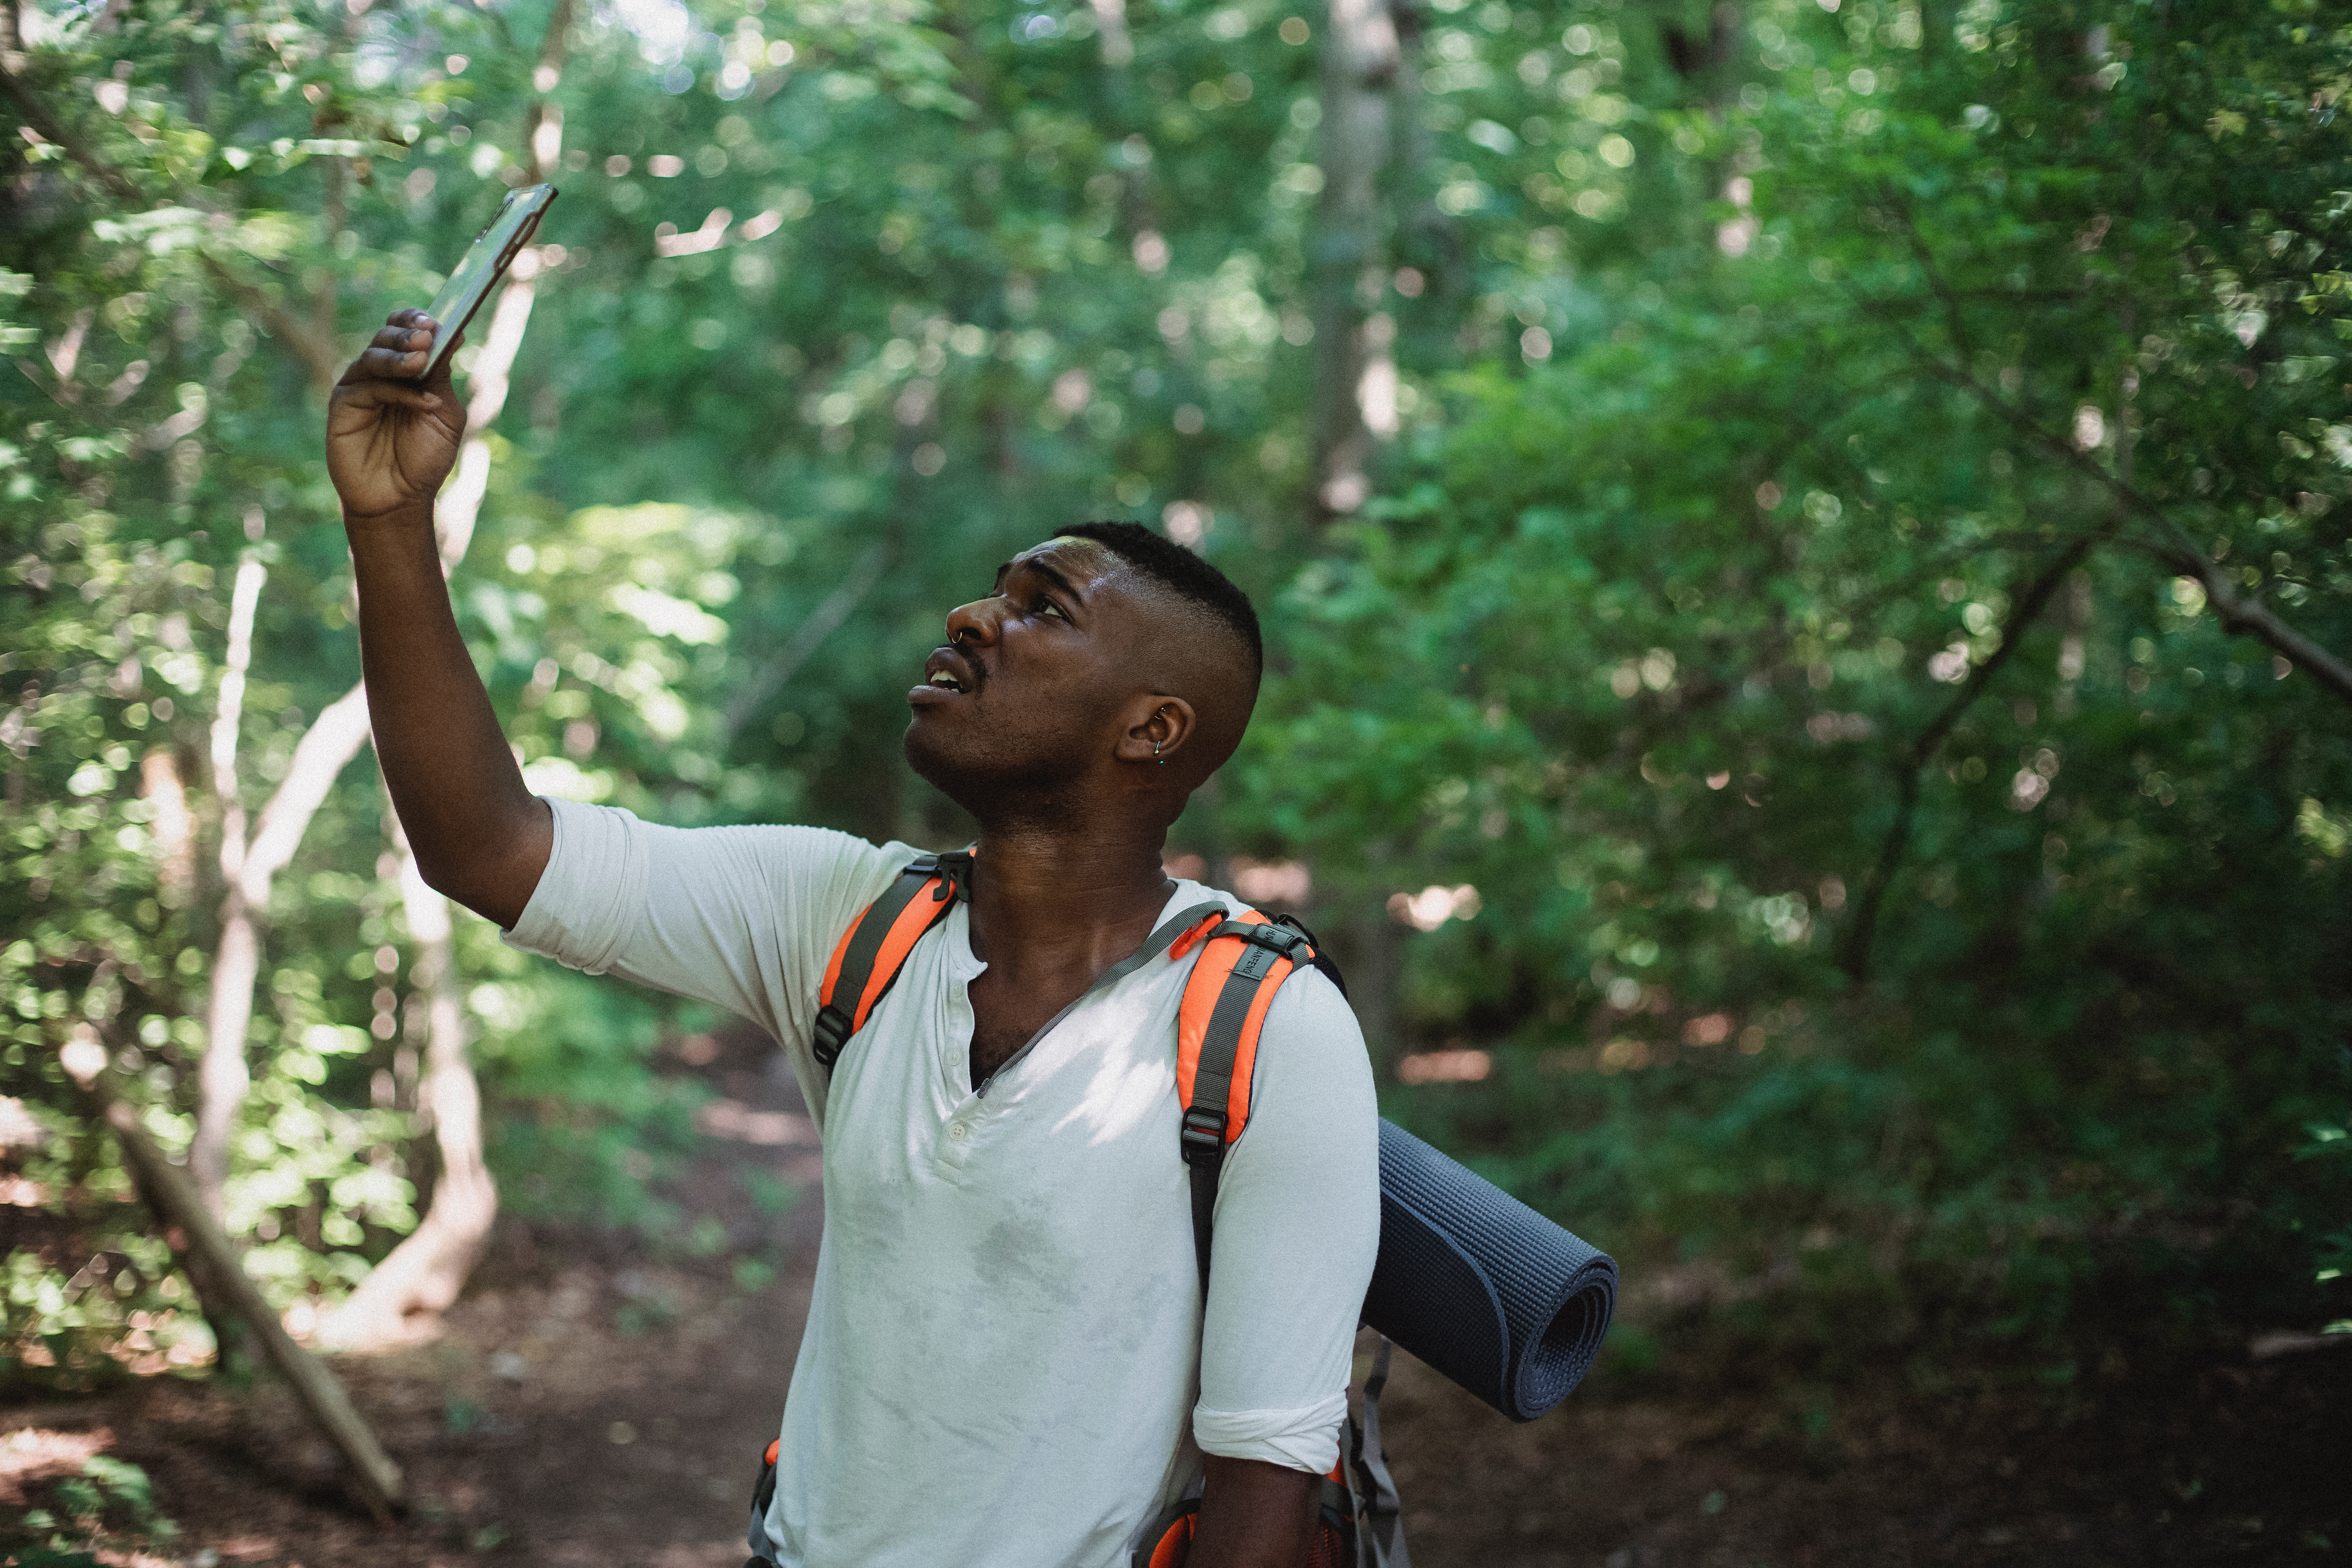
\includegraphics[width=0.6\textwidth]{media/no_internet.jpg}
	\end{figure}
\end{frame}
\begin{frame}   
	\frametitle{Situation 2: low battery}
	 \begin{figure}
		\centering
		\includegraphics[width=0.4\textwidth]{media/low_battery.jpg}
	\end{figure}
\end{frame}




\section{Situation 1:  Offline Challenge}
\begin{frame}   
	\frametitle{Situation 1:  Storyboard}
	\begin{columns}
	  \column{0.3\linewidth} 
		\begin{itemize}
			\item Persona: Fred Flintstone, Student
			\item Scenario: Check event information on the go
		\end{itemize}
		 \column{0.45\linewidth}   
		 \begin{figure}
			\centering
			\includegraphics[width=1\textwidth]{media/storyboard1.jpg}
		\end{figure}
	\end{columns}
\end{frame}

\begin{frame}
	\frametitle{Situation 1: Context Model}
	 \begin{figure}
		\centering
		\includegraphics[width=0.7\textwidth]{media/contextmodel1.jpg}
	\end{figure}
\end{frame}

\begin{frame}   
	\frametitle{Situation 1: MAPE-K}
	\begin{itemize}
		\item Monitor: Network state, Package loss, Bandwidth
		\item Analyze: 
			 \begin{itemize} 
				\item Case 1: No connection
				\item Case 2: Stable connection
			\end{itemize}
		\item Plan:
			\begin{itemize}
				\item Case 1: use cached data 
				\item Case 2:  update data
			\end{itemize}
		\item Execute:
			\begin{itemize}
				\item Case 1: load cached data, ignore online messages
    				\item Case 2: send requests for updates, fetch only web data 
			\end{itemize}
		\item Knowledge: Store behavior model in Android Preferences
	\end{itemize}
\end{frame}




\section{Situation 2:  Energy Challenge}
\begin{frame}   
	\frametitle{Situation 2:  Storyboard}
	\begin{columns}
	  \column{0.3\linewidth} 
		\begin{itemize}
			\item Persona: Martina Rina, Car Mechanic
			\item Scenario: Low battery status
		\end{itemize}
		 \column{0.45\linewidth}   
		 \begin{figure}
			\centering
			\includegraphics[width=1\textwidth]{media/storyboard2.jpg}
		\end{figure}
	\end{columns}
\end{frame}

\begin{frame}
	\frametitle{Situation 2: Context Model}
	 \begin{figure}
		\centering
		\includegraphics[width=0.7\textwidth]{media/contextmodel2.jpg}
	\end{figure}
\end{frame}

\begin{frame}   
	\frametitle{Situation 1: MAPE-K}
	\begin{itemize}
		\item Monitor: Batterie state, cpu usage while using it
		\item Analyze: 
			 \begin{itemize} 
				\item Case 1: batterie state $<$ LOW \&\& batterie state $>$ CRITICAL
				\item Case 1: batterie state $<$ LOW \&\& batterie state $<$ CRITICAL
				\item Case 1: batterie state $>$ LOW \&\& batterie state $<$ CRITICAL
			\end{itemize}
		\item Plan:
			\begin{itemize}
				\item Case 1: limit gps, fetch only important data 
				\item Case 2: no gps, only cached data
				\item Case 3: use ACCESS\_FINE\_LOCATION for GPS, fetch data if possible
			\end{itemize}
		\item Execute:
			\begin{itemize}
				\item Case 1: set permission to ACCESS\_COARSE\_LOCATION, use cached data for unimportant things
    				\item Case 2: revoke permissions
    				\item Case 3: set ACCESS\_FINE\_LOCATION for GPS, grant every Internet permission
			\end{itemize}
		\item Knowledge: Store permissions in user preferences
	\end{itemize}
\end{frame}





\section{Detailed Architecture and Technology Choice}
\begin{frame}
	\frametitle{Detailed architecture and technology choice}
	 \begin{figure}
		\centering
		\includegraphics[width=0.8\textwidth]{media/architecture.jpg}
	\end{figure}
\end{frame}

\begin{frame}
	\frametitle{Detailed architecture and technology choice}
	 \begin{figure}
		\centering
		\includegraphics[width=1\textwidth]{media/entity-relationship-diagram.pdf}
	\end{figure}
\end{frame}

\end{document}